\section{Codevervollständigung}
\label{sec:codecompletion}
Sind in einem Projekt die Anforderungen definiert und von Hand erste Modelle und Architekturen entworfen, müssen diese implementiert werden. Dieses Kapitel behandelt die automatische und intelligente Codevervollständigung in Integrierten Entwicklungsumgebungen, also die Unterstützung während diesem Vorgang. 

\subsection{Allgemeine Konzepte}
\label{subsec:completion_concepts}
Automatische Codevervollständigung ist heutzutage in nahezu allen IDEs vorhanden. Es ist eines der meistgenutztesten Features von Softwareentwicklern \cite{MurphyKerstenFindlater2006}. Anhand verschiedener Ansätze werden dabei wahrscheinliche Vervollständigungen vorgeschlagen. Diese bestehen aus verschiedenen Dingen und variieren je nach Sprache. Übliche Vorschläge sind aber beispielsweise im Kontext verfügbare \textit{Methoden, Events, Klassen, Interfaces, Strukturen, Enums, Schlüsselwörter, lokale Variablen, Parameter oder Attribute, Dateien, Farben und Datentypen}. Durch verschiedene Methoden wird die Wahrscheinlichkeit dieser berechnet und in der Regel anhand einer Textbox zur Auswahl gestellt. Alternativ wird die wahrscheinlichste Option direkt ausgegraut angezeigt und kann beispielsweise durch die Tab-Taste akzeptiert werden. \autoref{fig:codecompletion} zeigt diese Optionen anhand von Visual Studio auf. 
\begin{figure}[!htb] 
	\centering
	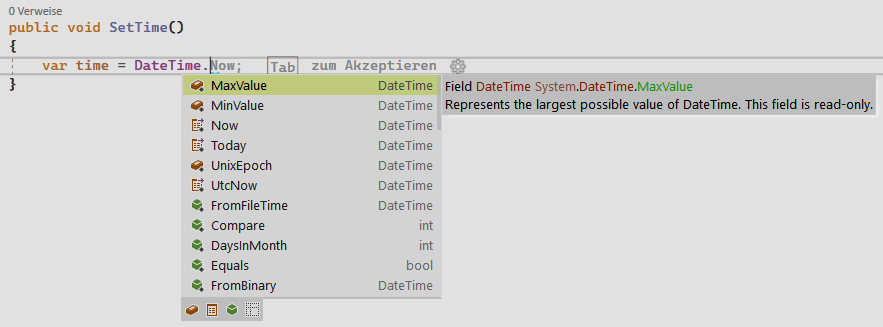
\includegraphics[width=125mm]{images/codecompletion.png}
	\caption{Code Vervollständigung in Visual Studio 2022}
	\label{fig:codecompletion}
\end{figure}
\FloatBarrier
Je mehr Zeichen bereits geschrieben wurden, desto genauer können die Vorschläge werden. Dies liegt daran, dass durch die schon geschriebenen Zeichen gewisse Optionen auszuschließen sind. Die Eingabe wird also ständig geparst und es ergeben sich mögliche Ergebnisse mit dem gleichen Präfix. Das Parsen kann beispielsweise durch reguläre Ausdrücke oder das Aufbauen von abstrakten Syntaxbäumen umgesetzt werden. Hierbei wird von der lexikalischen Analyse gesprochen. Ein anderer klassischer Ansatz ist die semantische Analyse. Diese verwendet ein Grammatikmodell der Sprache um anhand definierter Regeln nur Methoden anzuzeigen, welche auch legal sind. Dabei werden beispielsweise private Methoden herausgefiltert, wenn auf diese kein Zugriff vorhanden ist \cite{MarasoiuChurchBlackwell2015}. In der Regel werden beide Analysearten verwendet. 

Die Bestimmung der besten Ergebnisse ist dann durch verschiedene Implementierungen umsetzbar. Einfachste Lösung ist die Sortierung nach alphabetischer Reihenfolge oder dem Zeitpunkt der letzten Modifikation einer Methode. Auch denkbar ist die Priorisierung nach Lokalität, also beispielsweise zuerst die aktuelle Klasse, dann das Projekt und zuletzt Imports \cite{HobbesLanza2008}. 

Naheliegend ist auch die Sortierung nach der Anzahl der bisherigen Verwendungen eines Vorschlages. Diese Arten zählen zu den statistischen. Auch diese erzielen heutzutage bessere Ergebnisse, da öffentliche Repositories die notwendigen Daten zur Verfügung stellen. Anhand dieser können die Auftrittswahrscheinlichkeiten verschiedener Elemente ausgelesen werden um somit bessere Vorschläge zu erzielen. Verwendung findet dabei beispielsweise das N-Gram-Modell. Dieses zählt die Vorkommen verschiedener Kombinationen aus N Elementen \cite{Rosenfeld2000}. Problematisch ist, dass diese Modelle nur Abhängigkeiten zwischen wenigen Elementen feststellen. Außerdem funktioniert es nur, wenn Statistiken zu allen Element-Kombinationen vorhanden sind. 

Moderne Systeme nutzen immer häufiger einen anderen Ansatz: Künstliche Intelligenz. Im Gegensatz zur statistischen Analyse werden nicht nur Statistiken gesammelt sondern anhand von Daten wiederkehrende Muster erkannt. Diese schaffen es besser umfangreichen Kontext miteinzubeziehen und auf in den Trainingsdaten nicht vorhandene Elemente zu reagieren. Zur genauen Umsetzung gibt es verschiedenste Optionen. In \cite{Scharrenburg2019CodeCW} werden einige der verwendbaren rekurrenten neuronalen Netze gegenüber gestellt. Erwähnenswert ist außerdem der Algorithmus Best-Matching-Neighbour, welcher sich als sehr effizient herausgestellt hat \cite{BruchMonperrusMezini2009}.

\subsection{Nutzen und Risiken}
\label{subsec:completion_risks}
Die Nutzung von Codevervollständigung bringt zahlreiche Vorteile mit sich. Der größte ist die Zeitersparnis. Diese unterscheidet sich je nach Effektivität des Tools. Statt dem Ausschreiben ganzer Methodenaufrufe reicht oftmals der erste Buchstabe. Selbst wenn der gesuchte Vorschlag erst an dritter Stelle ist, muss nur zweimal die Pfeiltaste zur Auswahl betätigt werden. Im schlimmsten Fall müssen bereits mehrere Buchstaben vorhanden sein, damit die gesuchte Empfehlung kommt. Trotzdem findet eine enorme Zeiteinsparung statt. Gleiches gilt auch für die anderen Elemente, wie Variablen und Co. Einige Tools sprechen von ca. 40\% weniger Tastaturanschlägen \cite{Kite}. 
Außerdem werden durch die Vorschläge Tipp- und Logikfehler vermieden. Syntaktisch oder semantisch nicht korrekte Eingaben rufen keine Vorschläge hervor. Wird stattdessen die Eingabe durch Vorschläge vervollständigt, kann von syntaktischer und semantischer Korrektheit ausgegangen werden. Ein weiterer Vorteil ist, dass kein Detailwissen mehr benötigt wird. Sobald in objektorientierten Sprachen beispielsweise ein Punkt hinter das Objekt gesetzt wurde, werden dessen zugreifbare Methoden und Felder angezeigt. Dabei wird in der Regel bereits gefiltert, ob eine Zuweisung oder nur ein Aufruf stattfindet. Findet ersteres statt, werden nur Methoden und Felder mit Rückgabewert angezeigt. Besonders bei Nutzung fremder Bibliotheken ist dies von großem Vorteil. Somit können selbst schlecht dokumentierte Anwendungen und Bibliotheken verwendet werden, sofern die Namen verständlich gewählt wurden. Durch die Nutzung von Inline-Dokumentation sind die jeweiligen Methoden oftmals sogar direkt in der IDE beschrieben. 
Neben dem Vermeiden von Logik-Fehlern helfen diese Tools bereits beim Formulieren der Logik. Beispielsweise wird bei Zuweisung eines Wertes an eine Variable automatisch erkannt, wenn der Datentyp nicht übereinstimmt. Daher folgt ein Vorschlag zum Casting der Eingabe. Bei verschiedenen Collection-Arten werden dagegen beispielsweise auf diese anwendbare Strukturen wie \lstinline|foreach| vorgeschlagen. Das Gerüst dieser kann automatisch vervollständigt werden. Ein weiteres Beispiel ist die Rückgabe in einer Methode. Wird das passende Keyword geschrieben, kommen beispielsweise Vorschläge aus lokalen Variablen mit dem passenden Rückgabetyp. Die Beispiele sind zahlreich.

Diese Vorteile müssen allerdings mit Vorsicht genutzt werden. Die automatische Vervollständigung verleitet beispielsweise dazu, Vorschläge blind anzunehmen und einfach davon auszugehen, dass die dahinterliegende Funktionalität passend ist. Besonders bei fremden Bibliotheken wäre es dagegen sinnvoll, dies zu überprüfen oder die technische Dokumentation zu studieren. Gegebenenfalls hat eine verwendete Methode besonders schlechte Performance, ist bereits veraltet oder nicht Thread-safe, dies wird aber für die Anwendung benötigt. Hier muss zwingend vorsichtig vorgegangen werden.

\subsection{Marktanalyse}
\label{subsec:completion_analyse}
Es gibt verschiedene Tools zur Nutzung mit mehreren Sprachen. Bezüglich Microsoft und Visual Studio wird \textbf{IntelliSense} bzw. \textbf{IntelliCode} verwendet. Dieses unterstützt JavaScript, TypeScript, JSON, HTML, CSS, SCSS, C++, C\#, J\#, Visual Basic, XML, XSLT, SQL. Bei Nutzung der IDE Visual Studio Code ermöglichen Erweiterungen außerdem dutzende weitere Sprachen. Es basiert auf tausenden Repositories, deren Qualität durch eine Mindestanzahl an Sternen sichergestellt werden soll. 

Ähnlich viele Sprachen in verschiedenen Editoren unterstützt die alleinstehende Anwendung \textbf{Kite}. Diese wurden anhand von über 25 Millionen Dateien trainiert und soll die Tastenanschläge um ca. 40\% reduzieren \cite{Kite}. 

Besonders erwähnenswert ist allerdings das Projekt \textbf{Tabnine}. Es handelt sich um eine moderne, sehr umfangreiche Erweiterung. Bezüglich der Funktion Codevervollständigung ist diese kostenlos. Unterstützt werden 20 verschiedene IDEs und folgende Sprachen: Angular, C, C++, C\#, CSS, Dart, Go, Haskell, HTML, Java, Javascript, Kotlin, Matlab, NodeJS, ObjectiveC, Perl, PHP, Pyhton, React, Ruby, Rust, Sass, Scala, Swift und Typescript. Erkennbar ist das definierte Ziel, nicht auf spezielle Sprachen beschränkt zu sein. Besonderheit ist außerdem die Möglichkeit eigene Modelle zu trainieren indem ausgewählte Repositories verbunden werden. Dies ermöglicht die optimalen Vorschläge bezogen auf spezielle Projekte. So kann beispielsweise der Programmierstil innerhalb eines Unternehmens besser miteinbezogen werden. Dazu muss allerdings die kostenpflichtige Version (12€ pro User je Monat) in Verwendung sein. 
\begin{figure}[!htb] 
	\centering
	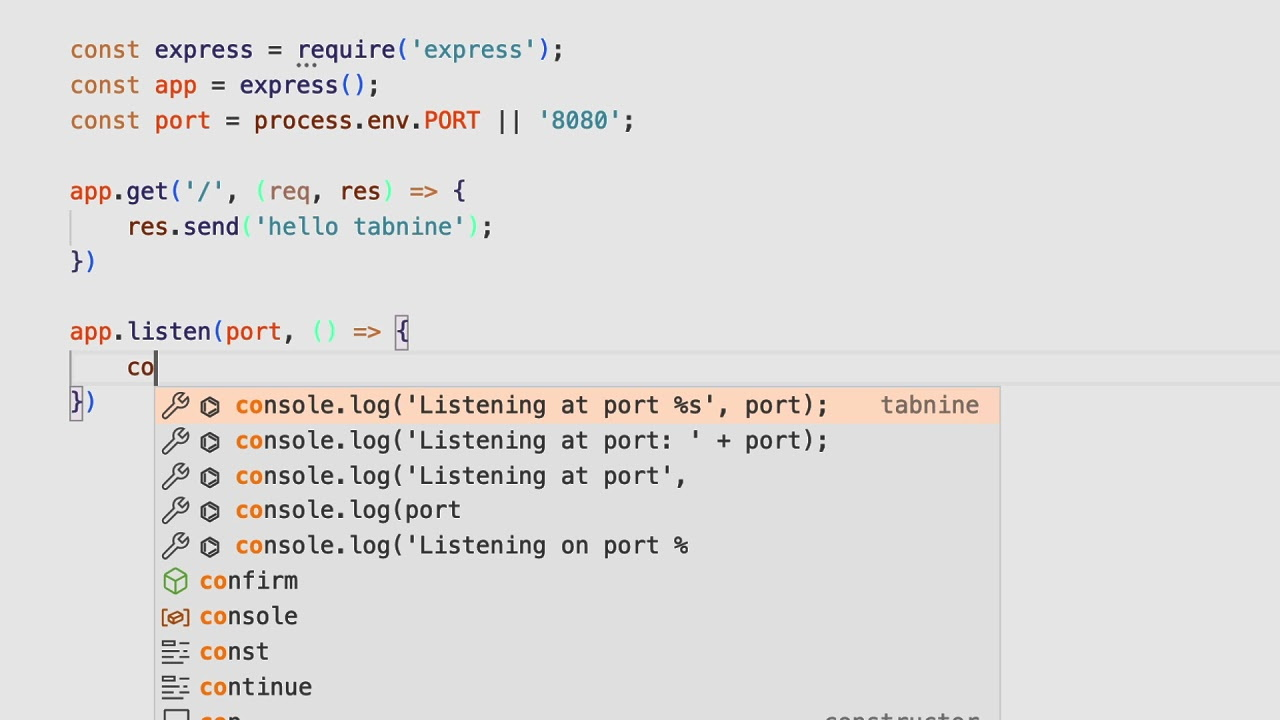
\includegraphics[width=125mm]{images/tabnine.jpg}
	\caption{Code Vervollständigung mit TabNine in VS Code}
	\label{fig:tabnine}
\end{figure}
\FloatBarrier
\autoref{fig:tabnine} zeigt die Vervollständigung durch TabNine in Visual Studio Code. Erkennbar ist, dass mehr als nur ein Methodenname vervollständigt wird. Anhand des Befehls \lstinline|app.listen(port, ...)| schlägt die Software einen passenden Text für das Logging unter Einbezug der Parameter vor. Als Grundlage von \textit{Tabnine} gilt das Modell GPT-2. Die verwendeten Daten stammen von GitHub-Repositories, für welche Qualität sichergestellt wurde. Neue Daten finden regelmäßig Einsatz im Training, um auch neuste Entwicklungen miteinzubeziehen.